% ── 10. Cost Considerations ───────────────────────────────────────────────────
\section{Cost Considerations}
\label{sec:cost}

Cost modelling for this system is driven by the portfolio of devices each user has deployed, their type of device (cameras, locks, thermostats), and the user's usage policies. To model cost, a monte carlo simulation was constructed that simulated user usage patterns. Pricing data from the AWS pricing calculator was used (Table~\ref{tab:pricing-constants}) to estimate cost.

\subsection{Simulation Methodology}

The Monte Carlo simulation was developed over a synthetic population of 1,000 households. Each household was assigned independent random draws for the following variables: a usage intensity scalar sampled from a clipped normal distribution (mean 0.5, standard deviation 0.2, bounded to the interval [0.05, 1.0]); a device count sampled uniformly from one to twelve non-camera modules; a camera adoption indicator (Bernoulli, 45\% probability) that, when positive, assigned one to four cameras to the household; a video retention policy sampled from a weighted discrete distribution favoring fourteen-day retention; a daily API call rate ranging from 15 to 250 calls linearly scaled by usage intensity; an IoT telemetry rate of 50 to 600 messages per device per day; a number of configured automation rules from zero to fifteen; and a notification opt-in flag (Bernoulli, 70\% probability). All downstream cost quantities were derived algebraically from these inputs using published AWS pricing for the us-east-1 region. No free-tier credits were applied, with the exception of Amazon Cognito, for which 1,000 monthly active users fall entirely within the 50,000-user free tier and therefore contribute no direct cost.

Table~\ref{tab:sim-inputs} enumerates the simulation input variables. The AWS pricing constants applied to each service are provided in Appendix~\ref{sec:appendix-pricing} (Table~\ref{tab:pricing-constants}).

\begin{table}[H]
  \centering
  \small
  \caption{Monte Carlo Simulation Input Variables}
  \label{tab:sim-inputs}
  \begin{tabular}{lll}
    \hline
    \textbf{Variable} & \textbf{Distribution} & \textbf{Parameters} \\
    \hline
    Usage intensity         & Normal (clipped)     & $\mu=0.50,\;\sigma=0.20,\;[0.05,\,1.0]$ \\
    Non-camera devices      & Discrete uniform     & $[1,\,12]$                                 \\
    Camera adoption         & Bernoulli            & $p=0.45$                                   \\
    Number of cameras       & Discrete uniform     & $[1,\,4]$ (camera users only)              \\
    Video retention         & Weighted categorical & 7\,d (25\%), 14\,d (40\%), 30\,d (25\%), 90\,d (10\%) \\
    Daily API calls         & Linear in usage      & $[15,\,250]$ calls/day                     \\
    IoT messages/device/day & Linear in usage      & $[50,\,600]$ messages/day                  \\
    Camera recording hrs/day & Linear in usage     & $[2,\,24]$ hours/day                      \\
    Camera viewing hrs/day  & Linear in usage      & $[0.1,\,2.0]$ hours/day                  \\
    Automation rules        & Linear in usage      & $[0,\,15]$ rules                         \\
    Notification opt-in     & Bernoulli            & $p=0.70$                                  \\
    \hline
  \end{tabular}
\end{table}

\subsection{Major Cost Drivers}
\begin{figure}[H]
  \centering
  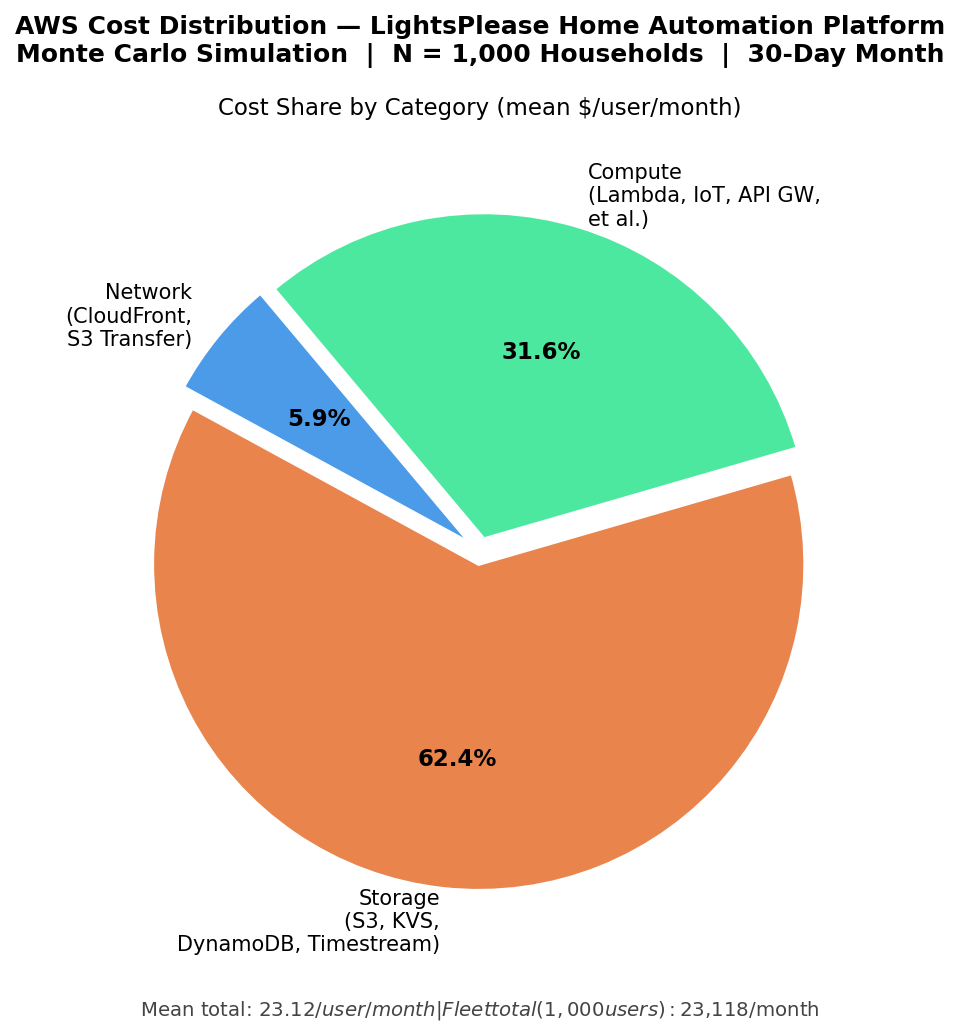
\includegraphics[width=0.5\linewidth]{../../data/cost_pie.png}
  \caption{Cost share by high-level category across 1,000 simulated households.}
  \label{fig:cost-pie}
\end{figure}

\begin{figure}[H]
  \centering
  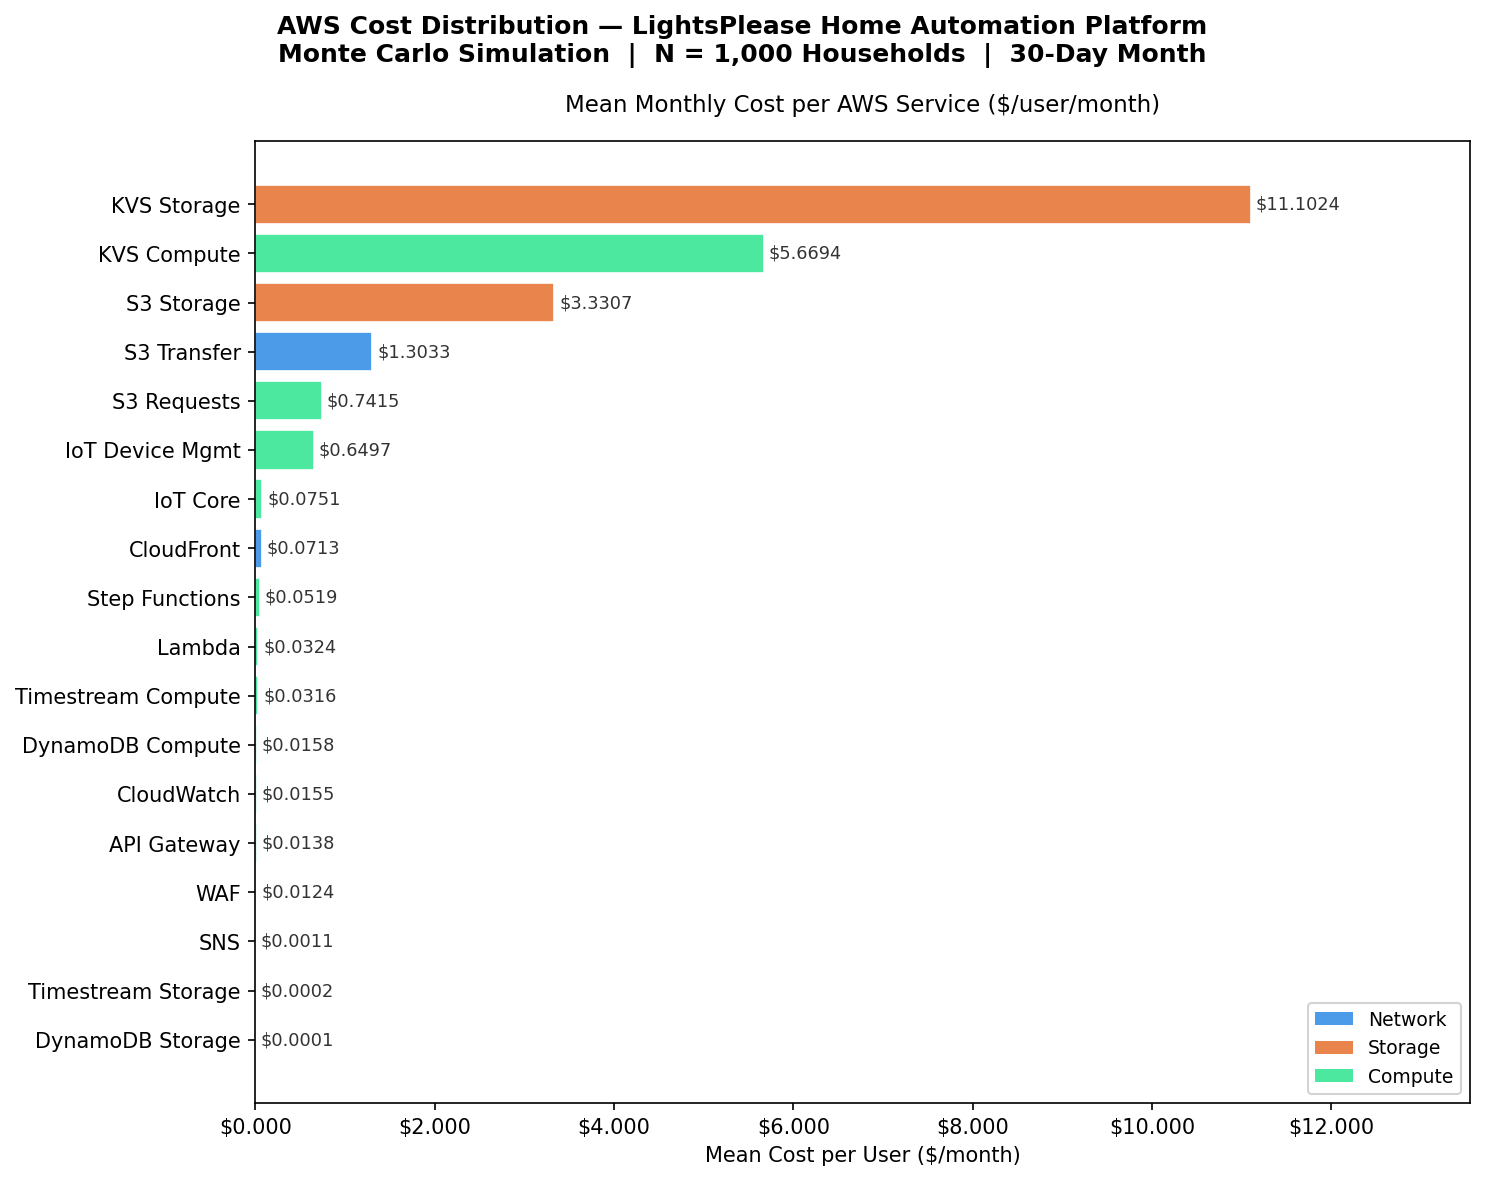
\includegraphics[width=0.75\linewidth]{../../data/cost_bar.png}
  \caption{Mean monthly cost per AWS service across 1,000 simulated households.}
  \label{fig:cost-bar}
\end{figure}

The simulation produced a mean total cost of \$23.12 per household per month across the 1,000-user population, equivalent to a fleet-wide cost of approximately \$23,100 per month, or \$277,400 per year, at this scale. Costs decompose into three high-level categories: storage at approximately 62\% of total spend, compute at approximately 32\%, and network egress at approximately 6\%.

Storage dominates the cost profile primarily because of Amazon Kinesis Video Streams. Camera-equipped households (45\% of the population) accumulate over 400 GB of video per camera per month at 1080p, making KVS retention the single largest line item and rendering the fleet average highly sensitive to camera adoption rate and default retention policies.

Within compute, AWS IoT Core and Lambda are the two largest contributors — IoT Core charges accrue from both device-connection minutes and message volume, while Lambda invocations are driven by the union of API calls, IoT-triggered processing, and automation rule evaluations. DynamoDB on-demand capacity adds further spend as each API call and roughly 10\% of IoT messages touch persistent state.

Network egress is comparatively modest. Static assets are served through CloudFront with aggressive caching, and the dominant egress cost is S3 retrieval for camera archival playback, which is limited because only approximately 10\% of stored video is retrieved during any billing period.

\subsection{Cost Scaling with Usage}

Device-side costs — IoT Core messages, IoT Device Management fleet indexing, and the associated Lambda processing — scale primarily with the number of registered devices per household and are largely fixed per user. Web-side costs — API Gateway, CloudFront, DynamoDB reads, and user-triggered Lambda invocations — scale with user engagement intensity and are more variable across the population; heavy users who check the application frequently or configure many automations spend measurably more per month than passive users with the same device count. Media costs — KVS ingest, KVS retention, and S3 archival — scale with camera count and recording hours and are by far the most volatile dimension; a household moving from one to four cameras with extended retention can increase its monthly cost by an order of magnitude relative to a non-camera household.

\subsection{Cost, Performance, and Reliability Tradeoffs}

DynamoDB was chosen to run in on-demand mode as an early-stage tradeoff to simplify deployment and guard against a risk of underprovisioning. As the fleet grows and traffic becomes more predictable, migrating high-traffic tables to provisioned capacity with auto-scaling would reduce DynamoDB spend significantly without sacrificing availability.

Kinesis Video Streams was selected over a direct-to-S3 camera pipeline specifically because it supports low-latency live streaming and provides a managed ingestion layer that removes the need for a custom media server. The cost of this capability is meaningfully higher than a deferred S3-only archival model, but it directly enables the live camera monitoring use case that is central to the product. A cost-reduction path would be to implement tiered storage: retain only the most recent 24 hours in KVS for live access and flush older footage to S3 Glacier Instant Retrieval for long-term archival at dramatically lower storage rates, at the cost of a slightly higher retrieval latency for older recordings.

AWS Lambda was chosen to run the backend processes as the pay-as-you-go model is suitable during periods of low activity — the platform incurs no compute charges when no requests are being processed — which is particularly favorable for a consumer home automation product where usage is concentrated in morning and evening windows rather than distributed uniformly across the day.
